\documentclass[a4paper, 11pt]{article}
\usepackage[top=3cm, bottom=3cm, left=2cm, right=2cm]{geometry}
\usepackage[utf8]{inputenc}
\usepackage{textcomp}
\usepackage{graphicx}
\usepackage{amsmath, amssymb}
\usepackage{bm}
\usepackage[pdftex, bookmarks, colorlinks, breaklinks]{hyperref}
\usepackage{memhfixc}
\usepackage{pdfsync}
\usepackage{fancyhdr}
\usepackage{fancyvrb}
\usepackage{fvextra}


\title{Rapport Base de Bonnées}
\author{Lucien Piat & Djemilatou Ouandaogo}

\begin{document}
\maketitle
\rule{8cm}{0.4pt}


\section{Introduction}
\subsection{Objectifs}
Ce projet vise à construire une base de données intégrant des données socio-économiques des départements et régions français entre 2008 et 2023. À travers l'utilisation de scripts Python et de requêtes SQL, notre objectif est de créer une base de donnée pour stocker, interroger et analyser ces données.

\subsection{Les avantages du modèle relationnel}
SQL est un langage de programmation utilisé pour gérer et manipuler des bases de données relationnelles.\\

Excel et les autres logiciels de gestion de données tabulaires, bien que très pratiques, présentent quelques limitations par rapport à SQL. Ils sont plus lents, ont des problèmes de portabilité, sont moins structurés et ne peuvent pas évoluer comme une base de données relationnelle. De plus, grâce au langage SQL, une infinité de requêtes peut être soumise à la base de données pour en tirer des informations détaillées.\\

Ainsi, lors de ce travail, nous inclurons les données de l'INSEE dans un modèle relationnel pour effectuer des requêtes sur ces dernières.\\
\subsection{Approche}
Tout d'abord, les données seront extraites des fichiers tabulaires et inscrites dans des DataFrames pandas. Elles seront ainsi triées pour faciliter leur utilisation et nettoyées. Nous enlèverons ainsi toutes les données inutiles à nos requêtes.\\

Dans un second temps, nous utiliserons un module de Python pour communiquer avec une base de données PostgreSQL. Nous créerons des tables qui seront ensuite remplies.\\

Finalement, nous créerons des requêtes pour répondre aux questions, un script pour parcourir les tables et un module de sauvegarde des données.\\
\section{Schéma de relation}
Voici le schéma de relation de notre base de données comprenant 5 tables.\\



\begin{figure}[h]
    \centering
    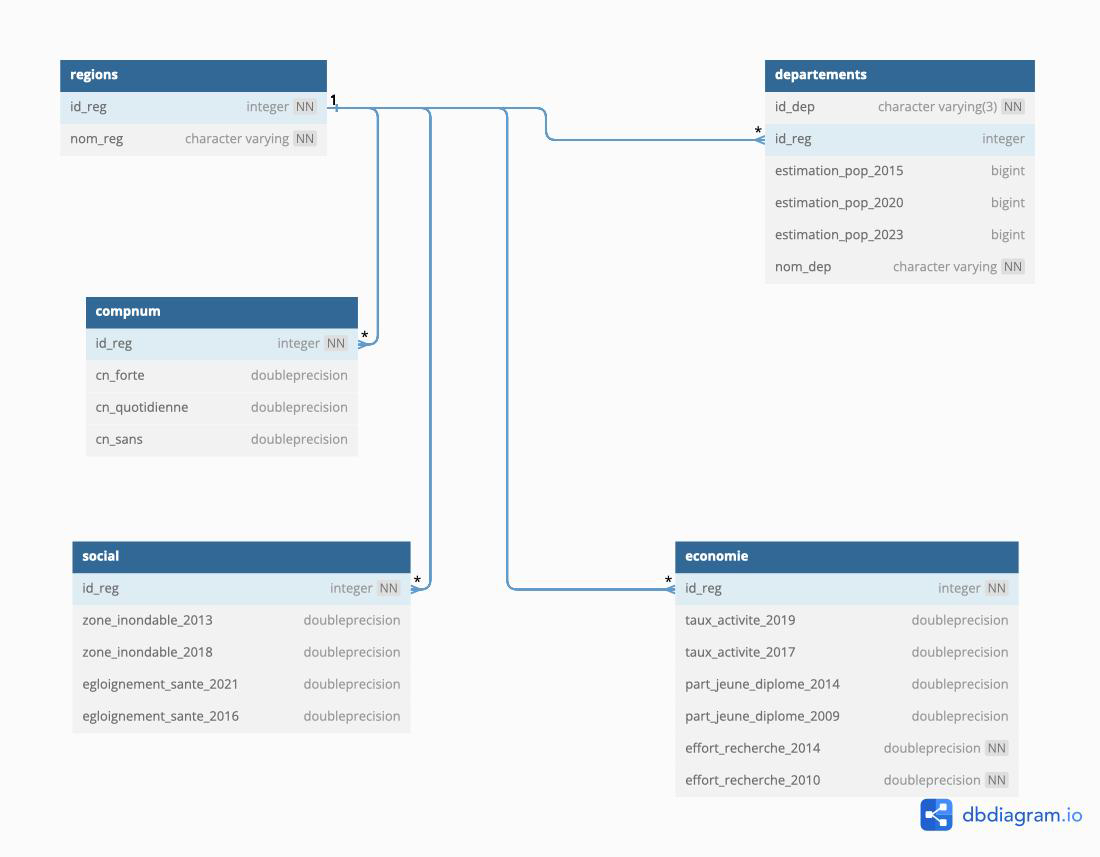
\includegraphics[width=0.85\textwidth]{Schema_BDD.jpg}
\end{figure}

\section{Explication sur vos choix de requêtes}
\subsection{Question 1}
\begin{Verbatim}[breaklines=true, breaksymbolleft=]
- `SELECT r.nom_reg, s.zone_inondable_2013`: Spécifie les colonnes à sélectionner dans le résultat. `r.nom_reg` représente le nom de la région, et `s.zone_inondable_2013` représente le taux de population habitant en zone inondable en 2013.

- `FROM public.Regions r JOIN public.Social s ON r.id_reg = s.id_reg`: Indique les tables à partir desquelles les données sont sélectionnées. Nous utilisons une jointure (JOIN) pour combiner les données des tables "Regions" (aliasée en tant que "r") et "Social" (aliasée en tant que "s"). Les tables sont jointes sur la colonne "id_reg", qui représente l'ID de la région.

- `WHERE s.zone_inondable_2013 > 10`: Filtre les lignes où le taux de population habitant en zone inondable en 2013 est supérieur à 10%.

- `ORDER BY s.zone_inondable_2013 DESC`: Trie les résultats.
\end{Verbatim}
\subsection{Question 2}
\begin{Verbatim}[breaklines=true, breaksymbolleft=]
- `SELECT r.nom_reg, (e.effort_recherche_2014 - e.effort_recherche_2010) AS variation_effort_recherche, e.taux_activite_2019`: Spécifie les colonnes à sélectionner dans le résultat. `r.nom_reg` représente le nom de la région. `(e.effort_recherche_2014 - e.effort_recherche_2010)` calcule la variation de l'effort de recherche et développement entre 2010 et 2014 et la renomme en tant que "variation_effort_recherche". `e.taux_activite_2019` représente le taux d'activité en 2019.

- `FROM public.Regions r JOIN public.CompNum c ON r.id_reg = c.id_reg JOIN public.Economie e ON r.id_reg = e.id_reg`: Indique les tables à partir desquelles les données sont sélectionnées. Nous utilisons des jointures pour combiner les données des tables "Regions", "CompNum" et "Economie". Les tables sont jointes sur la colonne "id_reg", qui représente l'ID de la région.

- `WHERE c.cn_quotidienne < 70`: Filtre les lignes en fonction d'une condition. Nous sélectionnons uniquement les régions où moins de 70% de la population a une utilisation quotidienne d'internet en 2019.

- `ORDER BY variation_effort_recherche`: Trie les résultats.
\end{Verbatim}
\subsection{Question 3}
\begin{Verbatim}[breaklines=true, breaksymbolleft=]
- `SELECT d.nom_dep, d.id_dep, (e.part_jeune_diplome_2014 - e.part_jeune_diplome_2009) AS evolution_jeunes_diplomes`: Spécifie les colonnes à sélectionner dans le résultat. `d.nom_dep` représente le nom du département, `d.id_dep` représente l'identifiant du département. `(e.part_jeune_diplome_2014 - e.part_jeune_diplome_2009)` calcule l'évolution de la part des jeunes diplômés entre 2009 et 2014.

- `FROM public.Departements d JOIN public.CompNum c ON d.id_reg = c.id_reg JOIN public.Economie e ON d.id_reg = e.id_reg`: Indique les tables à partir desquelles les données sont sélectionnées. Nous utilisons des jointures pour combiner les données des tables "Departements", "CompNum" et "Economie".

- `WHERE c.cn_forte < 25`: Filtre les lignes. 

- `ORDER BY evolution_jeunes_diplomes`: Trie les résultats.
\end{Verbatim}
\subsection{Question 4}
\begin{Verbatim}[breaklines=true, breaksymbolleft=]
- `SELECT d.nom_dep, d.estimation_pop_2020`: Spécifie les colonnes à sélectionner dans le résultat.

- `FROM public.Departements d JOIN public.CompNum c ON d.id_reg = c.id_reg`: Indique les tables à partir desquelles les données sont sélectionnées.

- `WHERE c.cn_forte >= 12.5`: Filtre les lignes. 
\end{Verbatim}
\subsection{Question 5}
\begin{Verbatim}[breaklines=true, breaksymbolleft=]
- `SELECT r.nom_reg, c.cn_quotidienne`: Spécifie les colonnes à sélectionner dans le résultat. 

- `FROM public.Regions r JOIN public.Social s ON r.id_reg = s.id_reg JOIN public.CompNum c ON r.id_reg = c.id_reg JOIN public.Economie e ON r.id_reg = e.id_reg`: Indique les tables à partir desquelles les données sont sélectionnées.

- `WHERE e.taux_activite_2019 > 75 AND s.egloignement_sante_2021 < 5`: Filtre les lignes en fonction de deux conditions. Nous sélectionnons uniquement les régions où le taux d'activité était supérieur à 75% en 2019 et où la part de la population éloignée de plus de 7 mn des services de santé de proximité était de moins de 5% en 2021.
\end{Verbatim}

\section{Conclusion}
Dans cet exercice, nous avons construit une base de données permettant de faciliter grandement la recherche sur les données de l'INSEE, qui étaient préalablement stockées dans plusieurs fichiers.\\

Cependant, nous n'utilisons qu'une fraction des données disponibles et pourrions les ajouter toutes pour étendre l'utilité du programme.\\

D'autre part, nous avons construit notre schéma de relation pour faciliter au maximum les requêtes, mais cela a rendu la gestion des années plus complexe. Il pourrait être cohérent de réviser ce point au risque d'ajouter de la redondance au profit de l'efficacité.\\

\end{document}